\chapter{Virtualisation}

\subsection{Introduction}

(one) Physical thing $\rightarrow$ Many Virtual thing\\

We are going to talk about virtualising:

\begin{itemize}
    \item CPU
    \item Memory
\end{itemize}

Virtualisation is an \textbf{Illusion}. It makes a running program
think that it has its own CPU and its own private memory.\\

Key aspects of Virtualisation:

\begin{itemize}
    \item Efficient: No point in making something if it performs
        worse than the trivial solution
    \item Secure: We might want to restrict the program to read
        only its data, and not some other program's data.
\end{itemize}

\section{CPU Virtualization}

one (or a few) CPUs $\rightarrow$ Many virtual CPUs\\

The way we are going to do is \textbf{time sharing}. We give each
program a little bit of time to use the cpu. We give A some time, 
the B some time, then C some time and then back to A. This is also
called multi-programming.\\

Abstraction: Process (running program)\\

Components of a process:

\begin{figure}[h!]
    \begin{center}
        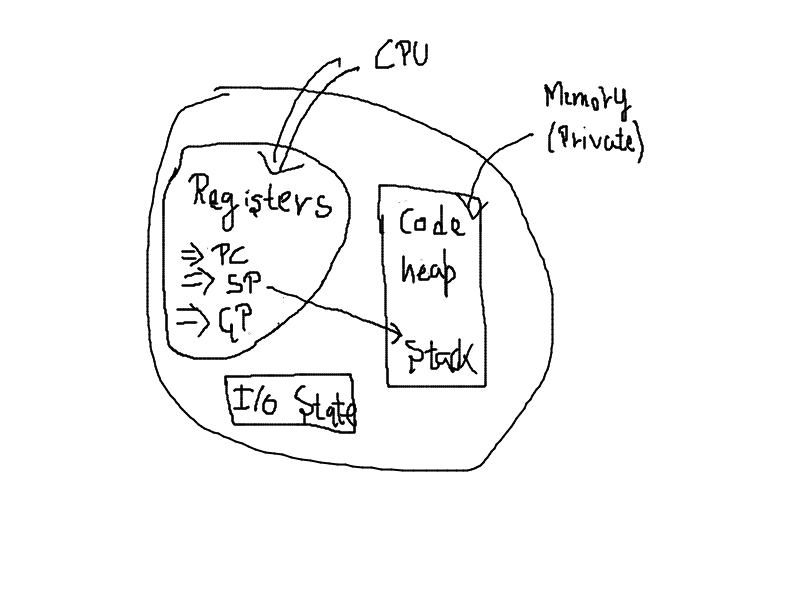
\includegraphics[width=8cm]{img/process.png}
        \caption{A process}
    \end{center}
\end{figure}

At the low-level there are \textbf{Mechanisms}:
How things work. You are
going to need some mechanisms to switch to other programs. You
also need some \textbf{Policies}:
High-level decisions which are built
on top of mechanisms.\\

Core mechanism behind all the cpu and memory virtualisation is
\textbf{Limited Direct Execution}.\\

The \textit{Direct Execution} part
directly pretains to efficency.\\

The \textit{Limited} part pretains to Security. The program
shouldn't have access to everything on the system.\\

\subsection{Direct Execution}

We havent defined what an OS is yet. Lets just say for now OS:
first program to run. We want to run a program "A".

\newpage

\begin{figure}[h!]
    \begin{center}
        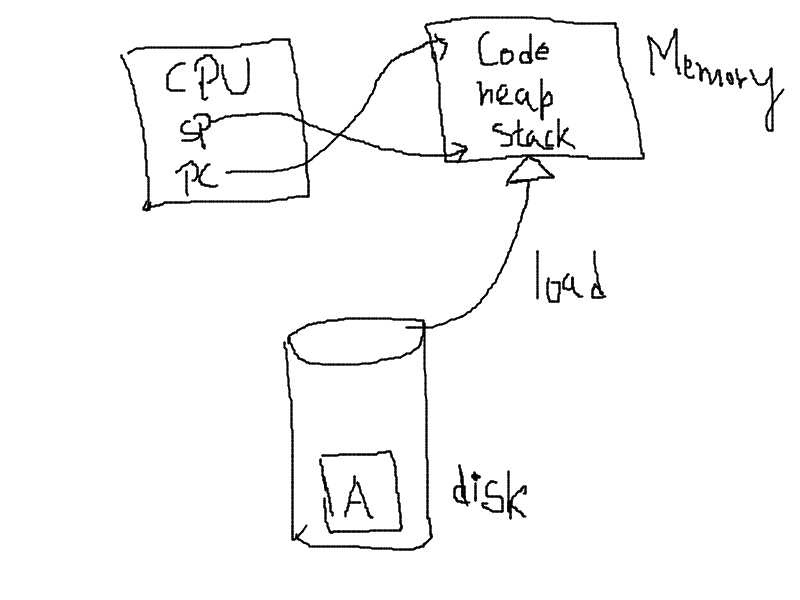
\includegraphics[width=8cm]{img/runprogram.png}
        \caption{Running a program}
    \end{center}
\end{figure}

Timeline: OS $\rightarrow$ A $\rightarrow \dots$\\

\textbf{Problems:}
\begin{itemize}
    \item What if "A" (user process) wants to do something
        \textit{restricted}?
    \item What if OS wants to stop "A", run "B"?
        (How does the OS regain control?)
    \item What if "A" does something that is slow? (Disk I/O)
\end{itemize}

\subsubsection{Problem 1: Restricted operation
(in a controlled way)}

Mode: per CPU bit.

\begin{itemize}
    \item OS: "kernal mode"\\
        This mode can do \textbf{anything}
    \item User program: "user mode"\\
        Can only do a limited number of things
\end{itemize}

Its a little bit stored on each (virtual) cpu.\\

How to get into one of these modes? How to transition?\\

@boottime: boot in kernal mode. The OS is the first program runs.
We are going to have trust on this program.\\

Want to run a user program: Special instruction that both:

\begin{enumerate}
    \item Transition into user mode
    \item Jumps in user program
\end{enumerate}

User program: Wants to do something restricted (example: disk I/O)

\begin{enumerate}
    \item Jump into kernal mode
    \item Jumps into kernal\\
        If you could jump into the kernal just like this then
        you could do anything you want. This can be a security
        issue. We want to be able to switch to kernal mode from 
        user mode but we dont want to allow to jump to any
        address in the kernal. We want to make this a restricted
        jump.
\end{enumerate}

Two instructions:

\begin{itemize}
    \item Trap\\
        Jump into the kernal (but @ restricted location) and then
        elevate "privilege" (use $\rightarrow$ kernal) also save
        enough register state so that we can return properly.
    \item Return from Trap
\end{itemize}

Timeline:\\

\begin{center}
    A $\xrightarrow{\text{trap}}$ OS $\rightarrow$ does some stuff
    $\xrightarrow{\text{return from trap}} \dots$ 
\end{center}

These traps are called \textbf{System Calls}\\

@boottime: OS starts up in kernal mode. It tells the hardware where
to jump to when somebody issues a kind of trap. For example, oh this
is trap number 80. When the OS sees this trap number, it has already
declared what trap number 80 is and jumps to what piece of code to
run.\\

Setup all these \textit{trap handlers}
issuing special instruction to tell hardware where trap handler
are in OS memory. Now, if someone issues a trap number, the OS
knows where to jump to, to execute the program.\\

We need to save/restore "state" (register) of process:\\

\begin{figure}[h!]
    \begin{center}
        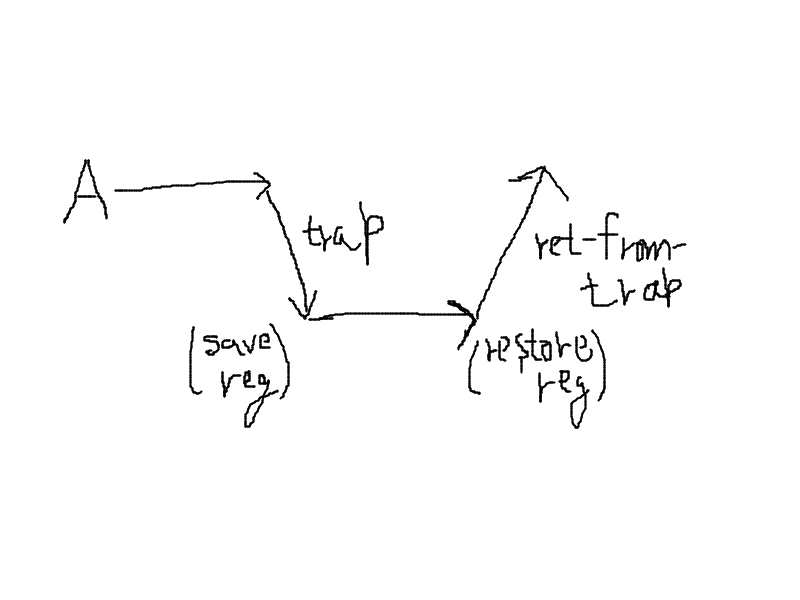
\includegraphics[width=5cm]{img/systemcall.png}
        \caption{A system call}
    \end{center}
\end{figure}

For you what it looks like when you call a trapis,
your execution was halted in mid
and something happened and you go to the instruction after the
trap.\\

\subsubsection{Problem 2: How to stop A,run B?}

OS was running $\rightarrow$ A $\rightarrow$ while(1);
$\rightarrow \dots$\\

cooperative approach: hope that A doesnt do bad stuff\\

non-cooperative (preemptive) approach: based on h/w support. H/w
support in this case is \textbf{timer interrupt}.\\

@boot: OS $\rightarrow$ kernal mode, installs trap handlers, starts
interrupt timer.

\begin{figure}[h!]
    \begin{center}
        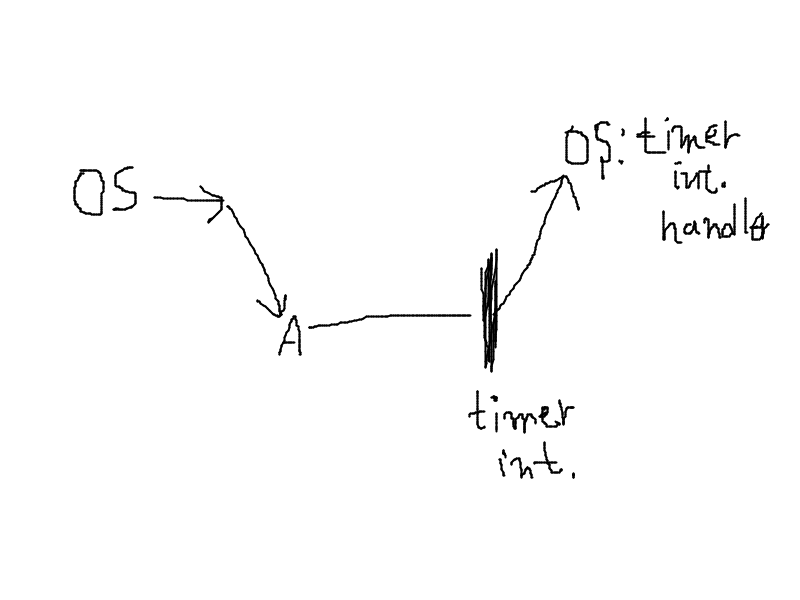
\includegraphics[width=5cm]{img/interupttimer.png}
        \caption{Interupt Timer}
    \end{center}
\end{figure}
